\documentclass[11pt,aspectratio=169]{beamer}
% =============================================================================
%  Shared Beamer preamble — Machine Learning I & II, PEU-CD 2026 (ENEI / INEI)
%
%  Inherited from the ML_Foundations deck (Alexander Quispe), with three changes:
%    * `minted` removed — it shells out to Pygments and does not build under
%      tectonic; every code block in the course uses `listings`.
%    * unused packages (lipsum, blindtext, multimedia, videoframe) dropped.
%    * `bbm` dropped — its fonts are PK-only and tectonic cannot render them;
%      the indicator uses \mathbf{1} instead.
%    * a math-macro block added so all twelve lectures share one notation.
%
%  Each lecture is a standalone document:
%      \documentclass[11pt,aspectratio=169]{beamer}
%      % =============================================================================
%  Shared Beamer preamble — Machine Learning I & II, PEU-CD 2026 (ENEI / INEI)
%
%  Inherited from the ML_Foundations deck (Alexander Quispe), with three changes:
%    * `minted` removed — it shells out to Pygments and does not build under
%      tectonic; every code block in the course uses `listings`.
%    * unused packages (lipsum, blindtext, multimedia, videoframe) dropped.
%    * `bbm` dropped — its fonts are PK-only and tectonic cannot render them;
%      the indicator uses \mathbf{1} instead.
%    * a math-macro block added so all twelve lectures share one notation.
%
%  Each lecture is a standalone document:
%      \documentclass[11pt,aspectratio=169]{beamer}
%      % =============================================================================
%  Shared Beamer preamble — Machine Learning I & II, PEU-CD 2026 (ENEI / INEI)
%
%  Inherited from the ML_Foundations deck (Alexander Quispe), with three changes:
%    * `minted` removed — it shells out to Pygments and does not build under
%      tectonic; every code block in the course uses `listings`.
%    * unused packages (lipsum, blindtext, multimedia, videoframe) dropped.
%    * `bbm` dropped — its fonts are PK-only and tectonic cannot render them;
%      the indicator uses \mathbf{1} instead.
%    * a math-macro block added so all twelve lectures share one notation.
%
%  Each lecture is a standalone document:
%      \documentclass[11pt,aspectratio=169]{beamer}
%      \input{../../../style/preamble}
% =============================================================================

% ---------- fonts ----------
\usepackage{helvet}
\usepackage[default]{lato}
\usepackage{tgbonum}
\usepackage{mathpazo}
\usepackage[utf8]{inputenc}

% ---------- math ----------
\usepackage{amsmath,amssymb}
\usepackage{mathtools}

% ---------- graphics, tables, layout ----------
\usepackage{graphicx}
\usepackage{tikz}
\usetikzlibrary{positioning,calc,arrows,arrows.meta,decorations.markings,shapes.misc,matrix,shapes,fit}
\usepackage{array}
\usepackage{booktabs}
\usepackage{multirow}
\usepackage{dcolumn}
\usepackage{subcaption}
\usepackage{caption}
\usepackage{changepage}
\usepackage{xspace}
\usepackage{tcolorbox}
\tcbuselibrary{skins,breakable}
\usepackage[ruled,vlined]{algorithm2e}
\usepackage{listings}
\usepackage{appendixnumberbeamer}
\usepackage{hyperref}

\newcolumntype{d}[0]{D{.}{.}{5}}
\setbeamertemplate{caption}[numbered]

% ---------- palette (Okabe–Ito, colour-blind safe) ----------
\definecolor{blue}{RGB}{0,114,178}
\definecolor{red}{RGB}{213,94,0}
\definecolor{yellow}{RGB}{240,228,66}
\definecolor{green}{RGB}{0,158,115}
\definecolor{MyBackground}{RGB}{255,253,218}

\hypersetup{colorlinks=true, linkbordercolor={white}, linkcolor={blue}, urlcolor={blue}}

% ---------- beamer look ----------
\setbeamercolor{frametitle}{fg=blue}
\setbeamercolor{title}{fg=black}
\setbeamertemplate{footline}[frame number]
\setbeamertemplate{navigation symbols}{}
\setbeamertemplate{itemize items}{-}
\setbeamercolor{itemize item}{fg=blue}
\setbeamercolor{itemize subitem}{fg=blue}
\setbeamercolor{enumerate item}{fg=blue}
\setbeamercolor{enumerate subitem}{fg=blue}
\setbeamercolor{button}{bg=MyBackground,fg=blue}
\setbeamercolor{section in toc}{fg=blue}
\setbeamercolor{subsection in toc}{fg=red}
\setbeamersize{text margin left=1em,text margin right=1em}
\setbeamercolor{block title}{fg=white,bg=blue}
\setbeamercolor{block body}{bg=blue!5}
\setbeamercolor{block title alerted}{fg=white,bg=red}
\setbeamercolor{block body alerted}{bg=red!5}
\setbeamercolor{block title example}{fg=white,bg=green}
\setbeamercolor{block body example}{bg=green!5}
\setbeamertemplate{blocks}[rounded][shadow=false]

\newenvironment{wideitemize}{\itemize\addtolength{\itemsep}{10pt}}{\enditemize}

\newenvironment{transitionframe}{
  \setbeamercolor{background canvas}{bg=yellow}
  \begin{frame}}{
  \end{frame}
}

% Section divider: a plain frame with a large blue title.
\newcommand{\sectionframe}[1]{%
  \section{#1}%
  \begin{frame}[plain]\vfill\begin{center}{\Huge\textcolor{blue}{#1}}\end{center}\vfill\end{frame}}

% ---------- proof / derivation environments ----------
% derivation: a boxed, step-by-step algebraic argument. Title is the claim.
\newtcolorbox{derivation}[1]{enhanced, colback=blue!3, colframe=blue, fonttitle=\bfseries,
  title={#1}, boxrule=0.6pt, left=4pt, right=4pt, top=3pt, bottom=3pt, arc=2pt}
% claim: a result to be proved (theorem / lemma / proposition).
\newtcolorbox{claim}[1]{enhanced, colback=white, colframe=black, fonttitle=\bfseries,
  title={#1}, boxrule=0.6pt, left=4pt, right=4pt, top=3pt, bottom=3pt, arc=2pt}
% keypoint: the one line to remember from a slide.
\newtcolorbox{keypoint}{enhanced, colback=green!6, colframe=green, boxrule=0.6pt,
  left=4pt, right=4pt, top=3pt, bottom=3pt, arc=2pt}
% caution: a common mistake or a subtlety.
\newtcolorbox{caution}{enhanced, colback=red!5, colframe=red, boxrule=0.6pt,
  left=4pt, right=4pt, top=3pt, bottom=3pt, arc=2pt}

% ---------- code ----------
\lstset{
  basicstyle=\ttfamily\scriptsize, keywordstyle=\color{blue}\bfseries,
  commentstyle=\color{green}, stringstyle=\color{red},
  showstringspaces=false, breaklines=true, frame=single, rulecolor=\color{black!30},
  numbers=none, xleftmargin=4pt, framexleftmargin=4pt, language=Python
}

\input{../../../style/macros}

% ---------- course-wide title metadata ----------
\newcommand{\courseinstitution}{ENEI -- INEI \,\textperiodcentered\, PEU-CD 2026}
\newcommand{\courseauthor}{Alexander Quispe}
\institute{\courseinstitution}
\author{\courseauthor}

% =============================================================================

% ---------- fonts ----------
\usepackage{helvet}
\usepackage[default]{lato}
\usepackage{tgbonum}
\usepackage{mathpazo}
\usepackage[utf8]{inputenc}

% ---------- math ----------
\usepackage{amsmath,amssymb}
\usepackage{mathtools}

% ---------- graphics, tables, layout ----------
\usepackage{graphicx}
\usepackage{tikz}
\usetikzlibrary{positioning,calc,arrows,arrows.meta,decorations.markings,shapes.misc,matrix,shapes,fit}
\usepackage{array}
\usepackage{booktabs}
\usepackage{multirow}
\usepackage{dcolumn}
\usepackage{subcaption}
\usepackage{caption}
\usepackage{changepage}
\usepackage{xspace}
\usepackage{tcolorbox}
\tcbuselibrary{skins,breakable}
\usepackage[ruled,vlined]{algorithm2e}
\usepackage{listings}
\usepackage{appendixnumberbeamer}
\usepackage{hyperref}

\newcolumntype{d}[0]{D{.}{.}{5}}
\setbeamertemplate{caption}[numbered]

% ---------- palette (Okabe–Ito, colour-blind safe) ----------
\definecolor{blue}{RGB}{0,114,178}
\definecolor{red}{RGB}{213,94,0}
\definecolor{yellow}{RGB}{240,228,66}
\definecolor{green}{RGB}{0,158,115}
\definecolor{MyBackground}{RGB}{255,253,218}

\hypersetup{colorlinks=true, linkbordercolor={white}, linkcolor={blue}, urlcolor={blue}}

% ---------- beamer look ----------
\setbeamercolor{frametitle}{fg=blue}
\setbeamercolor{title}{fg=black}
\setbeamertemplate{footline}[frame number]
\setbeamertemplate{navigation symbols}{}
\setbeamertemplate{itemize items}{-}
\setbeamercolor{itemize item}{fg=blue}
\setbeamercolor{itemize subitem}{fg=blue}
\setbeamercolor{enumerate item}{fg=blue}
\setbeamercolor{enumerate subitem}{fg=blue}
\setbeamercolor{button}{bg=MyBackground,fg=blue}
\setbeamercolor{section in toc}{fg=blue}
\setbeamercolor{subsection in toc}{fg=red}
\setbeamersize{text margin left=1em,text margin right=1em}
\setbeamercolor{block title}{fg=white,bg=blue}
\setbeamercolor{block body}{bg=blue!5}
\setbeamercolor{block title alerted}{fg=white,bg=red}
\setbeamercolor{block body alerted}{bg=red!5}
\setbeamercolor{block title example}{fg=white,bg=green}
\setbeamercolor{block body example}{bg=green!5}
\setbeamertemplate{blocks}[rounded][shadow=false]

\newenvironment{wideitemize}{\itemize\addtolength{\itemsep}{10pt}}{\enditemize}

\newenvironment{transitionframe}{
  \setbeamercolor{background canvas}{bg=yellow}
  \begin{frame}}{
  \end{frame}
}

% Section divider: a plain frame with a large blue title.
\newcommand{\sectionframe}[1]{%
  \section{#1}%
  \begin{frame}[plain]\vfill\begin{center}{\Huge\textcolor{blue}{#1}}\end{center}\vfill\end{frame}}

% ---------- proof / derivation environments ----------
% derivation: a boxed, step-by-step algebraic argument. Title is the claim.
\newtcolorbox{derivation}[1]{enhanced, colback=blue!3, colframe=blue, fonttitle=\bfseries,
  title={#1}, boxrule=0.6pt, left=4pt, right=4pt, top=3pt, bottom=3pt, arc=2pt}
% claim: a result to be proved (theorem / lemma / proposition).
\newtcolorbox{claim}[1]{enhanced, colback=white, colframe=black, fonttitle=\bfseries,
  title={#1}, boxrule=0.6pt, left=4pt, right=4pt, top=3pt, bottom=3pt, arc=2pt}
% keypoint: the one line to remember from a slide.
\newtcolorbox{keypoint}{enhanced, colback=green!6, colframe=green, boxrule=0.6pt,
  left=4pt, right=4pt, top=3pt, bottom=3pt, arc=2pt}
% caution: a common mistake or a subtlety.
\newtcolorbox{caution}{enhanced, colback=red!5, colframe=red, boxrule=0.6pt,
  left=4pt, right=4pt, top=3pt, bottom=3pt, arc=2pt}

% ---------- code ----------
\lstset{
  basicstyle=\ttfamily\scriptsize, keywordstyle=\color{blue}\bfseries,
  commentstyle=\color{green}, stringstyle=\color{red},
  showstringspaces=false, breaklines=true, frame=single, rulecolor=\color{black!30},
  numbers=none, xleftmargin=4pt, framexleftmargin=4pt, language=Python
}

% =============================================================================
%  Notation — one convention for all lectures
%
%  scalars      x, y, w           plain italic
%  vectors      \vx \vy \vw       bold lower-case
%  matrices     \vX \vW \vSigma   bold upper-case
%  parameters   \vbeta \vtheta    bold Greek
%  transpose    \vX\T             \top
% =============================================================================
\newcommand{\R}{\mathbb{R}}
\newcommand{\E}{\mathbb{E}}
\newcommand{\Prob}{\mathbb{P}}
\DeclareMathOperator{\Var}{Var}
\DeclareMathOperator{\Cov}{Cov}
\DeclareMathOperator{\tr}{tr}
\DeclareMathOperator{\diag}{diag}
\DeclareMathOperator{\rank}{rank}
\DeclareMathOperator{\sign}{sign}
\DeclareMathOperator{\col}{col}
\DeclareMathOperator{\RSS}{RSS}
\DeclareMathOperator*{\argmin}{arg\,min}
\DeclareMathOperator*{\argmax}{arg\,max}
\newcommand{\norm}[1]{\left\lVert #1 \right\rVert}
\newcommand{\abs}[1]{\left\lvert #1 \right\rvert}
\newcommand{\inner}[2]{\left\langle #1,\, #2 \right\rangle}
\newcommand{\ind}[1]{\mathbf{1}\!\left\{#1\right\}}
\newcommand{\T}{^{\top}}
\newcommand{\inv}{^{-1}}
\newcommand{\half}{\tfrac{1}{2}}
\newcommand{\eps}{\varepsilon}
\newcommand{\Dset}{\mathcal{D}}
\newcommand{\Hset}{\mathcal{H}}
\newcommand{\Lcal}{\mathcal{L}}
\newcommand{\Ncal}{\mathcal{N}}

% bold vectors
\newcommand{\vx}{\mathbf{x}}   \newcommand{\vy}{\mathbf{y}}   \newcommand{\vz}{\mathbf{z}}
\newcommand{\vw}{\mathbf{w}}   \newcommand{\vu}{\mathbf{u}}   \newcommand{\vv}{\mathbf{v}}
\newcommand{\vb}{\mathbf{b}}   \newcommand{\vh}{\mathbf{h}}   \newcommand{\vr}{\mathbf{r}}
\newcommand{\vc}{\mathbf{c}}   \newcommand{\vf}{\mathbf{f}}   \newcommand{\vg}{\mathbf{g}}
\newcommand{\vp}{\mathbf{p}}   \newcommand{\vq}{\mathbf{q}}   \newcommand{\vs}{\mathbf{s}}
\newcommand{\va}{\mathbf{a}}   \newcommand{\vd}{\mathbf{d}}   \newcommand{\vt}{\mathbf{t}}
\newcommand{\vk}{\mathbf{k}}   \newcommand{\vm}{\mathbf{m}}   \newcommand{\vn}{\mathbf{n}}
\newcommand{\vzero}{\mathbf{0}} \newcommand{\vone}{\mathbf{1}}
% bold matrices
\newcommand{\vX}{\mathbf{X}}   \newcommand{\vY}{\mathbf{Y}}   \newcommand{\vZ}{\mathbf{Z}}
\newcommand{\vW}{\mathbf{W}}   \newcommand{\vH}{\mathbf{H}}   \newcommand{\vI}{\mathbf{I}}
\newcommand{\vA}{\mathbf{A}}   \newcommand{\vB}{\mathbf{B}}   \newcommand{\vC}{\mathbf{C}}
\newcommand{\vD}{\mathbf{D}}   \newcommand{\vP}{\mathbf{P}}   \newcommand{\vQ}{\mathbf{Q}}
\newcommand{\vU}{\mathbf{U}}   \newcommand{\vV}{\mathbf{V}}   \newcommand{\vS}{\mathbf{S}}
\newcommand{\vM}{\mathbf{M}}   \newcommand{\vK}{\mathbf{K}}   \newcommand{\vG}{\mathbf{G}}
% bold Greek
\newcommand{\vbeta}{\boldsymbol{\beta}}     \newcommand{\valpha}{\boldsymbol{\alpha}}
\newcommand{\vtheta}{\boldsymbol{\theta}}   \newcommand{\vmu}{\boldsymbol{\mu}}
\newcommand{\vSigma}{\boldsymbol{\Sigma}}   \newcommand{\vLambda}{\boldsymbol{\Lambda}}
\newcommand{\veps}{\boldsymbol{\varepsilon}} \newcommand{\vphi}{\boldsymbol{\phi}}
\newcommand{\vgamma}{\boldsymbol{\gamma}}   \newcommand{\vlambda}{\boldsymbol{\lambda}}
\newcommand{\vdelta}{\boldsymbol{\delta}}   \newcommand{\vnu}{\boldsymbol{\nu}}
\newcommand{\vxi}{\boldsymbol{\xi}}         \newcommand{\vpi}{\boldsymbol{\pi}}
\newcommand{\vomega}{\boldsymbol{\omega}}



% ---------- course-wide title metadata ----------
\newcommand{\courseinstitution}{ENEI -- INEI \,\textperiodcentered\, PEU-CD 2026}
\newcommand{\courseauthor}{Alexander Quispe}
\institute{\courseinstitution}
\author{\courseauthor}

% =============================================================================

% ---------- fonts ----------
\usepackage{helvet}
\usepackage[default]{lato}
\usepackage{tgbonum}
\usepackage{mathpazo}
\usepackage[utf8]{inputenc}

% ---------- math ----------
\usepackage{amsmath,amssymb}
\usepackage{mathtools}

% ---------- graphics, tables, layout ----------
\usepackage{graphicx}
\usepackage{tikz}
\usetikzlibrary{positioning,calc,arrows,arrows.meta,decorations.markings,shapes.misc,matrix,shapes,fit}
\usepackage{array}
\usepackage{booktabs}
\usepackage{multirow}
\usepackage{dcolumn}
\usepackage{subcaption}
\usepackage{caption}
\usepackage{changepage}
\usepackage{xspace}
\usepackage{tcolorbox}
\tcbuselibrary{skins,breakable}
\usepackage[ruled,vlined]{algorithm2e}
\usepackage{listings}
\usepackage{appendixnumberbeamer}
\usepackage{hyperref}

\newcolumntype{d}[0]{D{.}{.}{5}}
\setbeamertemplate{caption}[numbered]

% ---------- palette (Okabe–Ito, colour-blind safe) ----------
\definecolor{blue}{RGB}{0,114,178}
\definecolor{red}{RGB}{213,94,0}
\definecolor{yellow}{RGB}{240,228,66}
\definecolor{green}{RGB}{0,158,115}
\definecolor{MyBackground}{RGB}{255,253,218}

\hypersetup{colorlinks=true, linkbordercolor={white}, linkcolor={blue}, urlcolor={blue}}

% ---------- beamer look ----------
\setbeamercolor{frametitle}{fg=blue}
\setbeamercolor{title}{fg=black}
\setbeamertemplate{footline}[frame number]
\setbeamertemplate{navigation symbols}{}
\setbeamertemplate{itemize items}{-}
\setbeamercolor{itemize item}{fg=blue}
\setbeamercolor{itemize subitem}{fg=blue}
\setbeamercolor{enumerate item}{fg=blue}
\setbeamercolor{enumerate subitem}{fg=blue}
\setbeamercolor{button}{bg=MyBackground,fg=blue}
\setbeamercolor{section in toc}{fg=blue}
\setbeamercolor{subsection in toc}{fg=red}
\setbeamersize{text margin left=1em,text margin right=1em}
\setbeamercolor{block title}{fg=white,bg=blue}
\setbeamercolor{block body}{bg=blue!5}
\setbeamercolor{block title alerted}{fg=white,bg=red}
\setbeamercolor{block body alerted}{bg=red!5}
\setbeamercolor{block title example}{fg=white,bg=green}
\setbeamercolor{block body example}{bg=green!5}
\setbeamertemplate{blocks}[rounded][shadow=false]

\newenvironment{wideitemize}{\itemize\addtolength{\itemsep}{10pt}}{\enditemize}

\newenvironment{transitionframe}{
  \setbeamercolor{background canvas}{bg=yellow}
  \begin{frame}}{
  \end{frame}
}

% Section divider: a plain frame with a large blue title.
\newcommand{\sectionframe}[1]{%
  \section{#1}%
  \begin{frame}[plain]\vfill\begin{center}{\Huge\textcolor{blue}{#1}}\end{center}\vfill\end{frame}}

% ---------- proof / derivation environments ----------
% derivation: a boxed, step-by-step algebraic argument. Title is the claim.
\newtcolorbox{derivation}[1]{enhanced, colback=blue!3, colframe=blue, fonttitle=\bfseries,
  title={#1}, boxrule=0.6pt, left=4pt, right=4pt, top=3pt, bottom=3pt, arc=2pt}
% claim: a result to be proved (theorem / lemma / proposition).
\newtcolorbox{claim}[1]{enhanced, colback=white, colframe=black, fonttitle=\bfseries,
  title={#1}, boxrule=0.6pt, left=4pt, right=4pt, top=3pt, bottom=3pt, arc=2pt}
% keypoint: the one line to remember from a slide.
\newtcolorbox{keypoint}{enhanced, colback=green!6, colframe=green, boxrule=0.6pt,
  left=4pt, right=4pt, top=3pt, bottom=3pt, arc=2pt}
% caution: a common mistake or a subtlety.
\newtcolorbox{caution}{enhanced, colback=red!5, colframe=red, boxrule=0.6pt,
  left=4pt, right=4pt, top=3pt, bottom=3pt, arc=2pt}

% ---------- code ----------
\lstset{
  basicstyle=\ttfamily\scriptsize, keywordstyle=\color{blue}\bfseries,
  commentstyle=\color{green}, stringstyle=\color{red},
  showstringspaces=false, breaklines=true, frame=single, rulecolor=\color{black!30},
  numbers=none, xleftmargin=4pt, framexleftmargin=4pt, language=Python
}

% =============================================================================
%  Notation — one convention for all lectures
%
%  scalars      x, y, w           plain italic
%  vectors      \vx \vy \vw       bold lower-case
%  matrices     \vX \vW \vSigma   bold upper-case
%  parameters   \vbeta \vtheta    bold Greek
%  transpose    \vX\T             \top
% =============================================================================
\newcommand{\R}{\mathbb{R}}
\newcommand{\E}{\mathbb{E}}
\newcommand{\Prob}{\mathbb{P}}
\DeclareMathOperator{\Var}{Var}
\DeclareMathOperator{\Cov}{Cov}
\DeclareMathOperator{\tr}{tr}
\DeclareMathOperator{\diag}{diag}
\DeclareMathOperator{\rank}{rank}
\DeclareMathOperator{\sign}{sign}
\DeclareMathOperator{\col}{col}
\DeclareMathOperator{\RSS}{RSS}
\DeclareMathOperator*{\argmin}{arg\,min}
\DeclareMathOperator*{\argmax}{arg\,max}
\newcommand{\norm}[1]{\left\lVert #1 \right\rVert}
\newcommand{\abs}[1]{\left\lvert #1 \right\rvert}
\newcommand{\inner}[2]{\left\langle #1,\, #2 \right\rangle}
\newcommand{\ind}[1]{\mathbf{1}\!\left\{#1\right\}}
\newcommand{\T}{^{\top}}
\newcommand{\inv}{^{-1}}
\newcommand{\half}{\tfrac{1}{2}}
\newcommand{\eps}{\varepsilon}
\newcommand{\Dset}{\mathcal{D}}
\newcommand{\Hset}{\mathcal{H}}
\newcommand{\Lcal}{\mathcal{L}}
\newcommand{\Ncal}{\mathcal{N}}

% bold vectors
\newcommand{\vx}{\mathbf{x}}   \newcommand{\vy}{\mathbf{y}}   \newcommand{\vz}{\mathbf{z}}
\newcommand{\vw}{\mathbf{w}}   \newcommand{\vu}{\mathbf{u}}   \newcommand{\vv}{\mathbf{v}}
\newcommand{\vb}{\mathbf{b}}   \newcommand{\vh}{\mathbf{h}}   \newcommand{\vr}{\mathbf{r}}
\newcommand{\vc}{\mathbf{c}}   \newcommand{\vf}{\mathbf{f}}   \newcommand{\vg}{\mathbf{g}}
\newcommand{\vp}{\mathbf{p}}   \newcommand{\vq}{\mathbf{q}}   \newcommand{\vs}{\mathbf{s}}
\newcommand{\va}{\mathbf{a}}   \newcommand{\vd}{\mathbf{d}}   \newcommand{\vt}{\mathbf{t}}
\newcommand{\vk}{\mathbf{k}}   \newcommand{\vm}{\mathbf{m}}   \newcommand{\vn}{\mathbf{n}}
\newcommand{\vzero}{\mathbf{0}} \newcommand{\vone}{\mathbf{1}}
% bold matrices
\newcommand{\vX}{\mathbf{X}}   \newcommand{\vY}{\mathbf{Y}}   \newcommand{\vZ}{\mathbf{Z}}
\newcommand{\vW}{\mathbf{W}}   \newcommand{\vH}{\mathbf{H}}   \newcommand{\vI}{\mathbf{I}}
\newcommand{\vA}{\mathbf{A}}   \newcommand{\vB}{\mathbf{B}}   \newcommand{\vC}{\mathbf{C}}
\newcommand{\vD}{\mathbf{D}}   \newcommand{\vP}{\mathbf{P}}   \newcommand{\vQ}{\mathbf{Q}}
\newcommand{\vU}{\mathbf{U}}   \newcommand{\vV}{\mathbf{V}}   \newcommand{\vS}{\mathbf{S}}
\newcommand{\vM}{\mathbf{M}}   \newcommand{\vK}{\mathbf{K}}   \newcommand{\vG}{\mathbf{G}}
% bold Greek
\newcommand{\vbeta}{\boldsymbol{\beta}}     \newcommand{\valpha}{\boldsymbol{\alpha}}
\newcommand{\vtheta}{\boldsymbol{\theta}}   \newcommand{\vmu}{\boldsymbol{\mu}}
\newcommand{\vSigma}{\boldsymbol{\Sigma}}   \newcommand{\vLambda}{\boldsymbol{\Lambda}}
\newcommand{\veps}{\boldsymbol{\varepsilon}} \newcommand{\vphi}{\boldsymbol{\phi}}
\newcommand{\vgamma}{\boldsymbol{\gamma}}   \newcommand{\vlambda}{\boldsymbol{\lambda}}
\newcommand{\vdelta}{\boldsymbol{\delta}}   \newcommand{\vnu}{\boldsymbol{\nu}}
\newcommand{\vxi}{\boldsymbol{\xi}}         \newcommand{\vpi}{\boldsymbol{\pi}}
\newcommand{\vomega}{\boldsymbol{\omega}}



% ---------- course-wide title metadata ----------
\newcommand{\courseinstitution}{ENEI -- INEI \,\textperiodcentered\, PEU-CD 2026}
\newcommand{\courseauthor}{Alexander Quispe}
\institute{\courseinstitution}
\author{\courseauthor}

\graphicspath{{figures/}}

\title{\textcolor{blue}{Lecture 6 \\ Unsupervised Learning: Clustering and PCA}}
\subtitle{Machine Learning I}
\date{September 28, 2026}

\begin{document}

\begin{frame}[plain]
\maketitle
\end{frame}

\begin{frame}{Outline}
\tableofcontents
\end{frame}

\begin{frame}{No Labels}
Five lectures on $\Dset=\{(\vx_i,y_i)\}$. Today $\Dset=\{\vx_i\}_{i=1}^N$, $\vx_i\in\R^p$, and nothing else.
\vspace{4pt}

Without a $y$ there is no loss $L(y,\hat y)$ and no test error. What replaces them is an \textbf{objective
defined on the inputs alone}, and the two classical ones are:
\begin{columns}[T]
\begin{column}{0.48\textwidth}
\textbf{Clustering}\\
Partition the points into $K$ groups so that points in a group are close and points in different groups are far.
Objective: within-group scatter.
\end{column}
\begin{column}{0.48\textwidth}
\textbf{Dimensionality reduction}\\
Map $\R^p\to\R^k$, $k\ll p$, losing as little as possible. Objective: reconstruction error, or retained variance.
\end{column}
\end{columns}
\vspace{8pt}
\begin{keypoint}
Both are optimization problems with exact statements and, for PCA, an exact solution. Neither has a
ground truth to compare against, so ``as little as possible'' must be defined before anything is computed.
\end{keypoint}
\end{frame}

% =============================================================================
\sectionframe{$k$-Means}
% =============================================================================

\begin{frame}{The Objective}
Assign each point to one of $K$ clusters, $c(i)\in\{1,\dots,K\}$, with centroids $\vmu_1,\dots,\vmu_K\in\R^p$.
\begin{block}{Within-cluster sum of squares}
\[
J(c,\vmu)=\sum_{i=1}^N\norm{\vx_i-\vmu_{c(i)}}^2=\sum_{k=1}^K\sum_{i:\,c(i)=k}\norm{\vx_i-\vmu_k}^2 .
\]
\end{block}
\begin{itemize}
  \item Minimizing over $c$ and $\vmu$ jointly is NP-hard, even for $K=2$ in the plane (Aloise et al., 2009).
  \item But for either variable \emph{with the other fixed} it is trivial. That is the algorithm.
\end{itemize}
\end{frame}

\begin{frame}{The Two Half-Steps}\small
\begin{derivation}{Fix $\vmu$, minimize over $c$}
The sum separates over $i$; the $i$-th term depends only on $c(i)$:
\[
c(i)=\argmin_k\norm{\vx_i-\vmu_k}^2 .
\]
Assign every point to its nearest centroid.
\end{derivation}
\begin{derivation}{Fix $c$, minimize over $\vmu$}
The sum separates over $k$. For cluster $k$ with $N_k$ members,
\[
\nabla_{\vmu_k}\sum_{i:\,c(i)=k}\norm{\vx_i-\vmu_k}^2=-2\sum_{i:\,c(i)=k}(\vx_i-\vmu_k)=\vzero
\quad\Longrightarrow\quad
\vmu_k=\frac1{N_k}\sum_{i:\,c(i)=k}\vx_i .
\]
Each centroid is the mean of its cluster --- hence the name.
\end{derivation}
Alternate the two until nothing changes. This is \textbf{coordinate descent} on $J$ (Lloyd, 1957).
\end{frame}

\begin{frame}{Numerical Example}\scriptsize
Six points in $\R^2$: $A(1,1)$, $B(1.5,2)$, $C(3,3.5)$, $D(5,7)$, $E(3.5,5)$, $F(4.5,5)$. Initial centroids $\vmu_1=A$, $\vmu_2=D$.
\begin{center}
\begin{tabular}{lcccccc|l}
\toprule
 & $A$ & $B$ & $C$ & $D$ & $E$ & $F$ & \\
\midrule
$\norm{\vx-\vmu_1}^2$, $\vmu_1=(1,1)$ & $0$ & $1.25$ & $10.25$ & $52$ & $22.25$ & $28.25$ & \\
$\norm{\vx-\vmu_2}^2$, $\vmu_2=(5,7)$ & $52$ & $37.25$ & $16.25$ & $0$ & $6.25$ & $4.25$ & \\
assignment & 1 & 1 & 1 & 2 & 2 & 2 & $J=11.5+10.5=22$ \\
\midrule
\multicolumn{7}{l}{update: $\vmu_1=\tfrac13(A+B+C)=(1.833,\,2.167)$, \quad $\vmu_2=\tfrac13(D+E+F)=(4.333,\,5.667)$} & \\
\midrule
$\norm{\vx-\vmu_1}^2$ & $2.06$ & $0.14$ & $3.14$ & $33.4$ & $10.8$ & $15.1$ & \\
$\norm{\vx-\vmu_2}^2$ & $32.9$ & $21.5$ & $6.47$ & $2.22$ & $1.14$ & $0.47$ & \\
assignment & 1 & 1 & 1 & 2 & 2 & 2 & $J=5.33+3.83=9.17$ \\
\bottomrule
\end{tabular}
\end{center}
No assignment changed in the second pass, so the centroids will not change either: converged, $J=9.17$.
% verify: L6.kmeans_example
\end{frame}

\begin{frame}{$k$-Means Converges}
\begin{claim}{Lloyd's algorithm terminates at a local minimum of $J$ in finitely many steps}
\end{claim}
\begin{derivation}{Proof}
\begin{itemize}
  \item Each half-step minimizes $J$ over one block of variables with the other fixed, so $J$ never increases:
        $J(c^{(t+1)},\vmu^{(t)})\le J(c^{(t)},\vmu^{(t)})$ and $J(c^{(t+1)},\vmu^{(t+1)})\le J(c^{(t+1)},\vmu^{(t)})$.
  \item $J\ge0$, so the non-increasing sequence $J^{(t)}$ converges.
  \item There are finitely many assignments $c$ (at most $K^N$), and each assignment determines its optimal $\vmu$.
        A strictly decreasing $J$ cannot revisit an assignment. So after finitely many steps no assignment changes,
        and the algorithm halts. \qed
\end{itemize}
\end{derivation}
\begin{caution}
``Local minimum'' is the operative phrase. Different initializations reach different partitions with
different $J$. Run it several times and keep the best; or initialize with care (next slide).
\end{caution}
\end{frame}

\begin{frame}{Initialization and Choosing $K$}\footnotesize
\begin{columns}[T]
\begin{column}{0.52\textwidth}
\textbf{$k$-means++} (Arthur \& Vassilvitskii, 2007)
\begin{enumerate}
  \item Pick $\vmu_1$ uniformly from the data.
  \item Pick $\vmu_{j+1}=\vx_i$ with probability $\propto\min_{l\le j}\norm{\vx_i-\vmu_l}^2$.
  \item Run Lloyd's algorithm.
\end{enumerate}
Far-apart seeds. Guarantee: $\E[J]\le8(\ln K+2)\,J^\star$ before Lloyd even starts.
\end{column}
\begin{column}{0.46\textwidth}
\textbf{Choosing $K$}
\begin{itemize}
  \item $J$ decreases in $K$ always ($K=N$ gives $J=0$). Look for the \emph{elbow} where the decrease slows.
  \item Silhouette: for each point, $(b-a)/\max(a,b)$ with $a$ its mean distance within its cluster and $b$ to the
        nearest other cluster. Average over points; pick $K$ maximizing it.
  \item Neither is a test error. Both are heuristics for a question the data cannot answer alone.
\end{itemize}
\end{column}
\end{columns}
\vspace{6pt}
\begin{center}
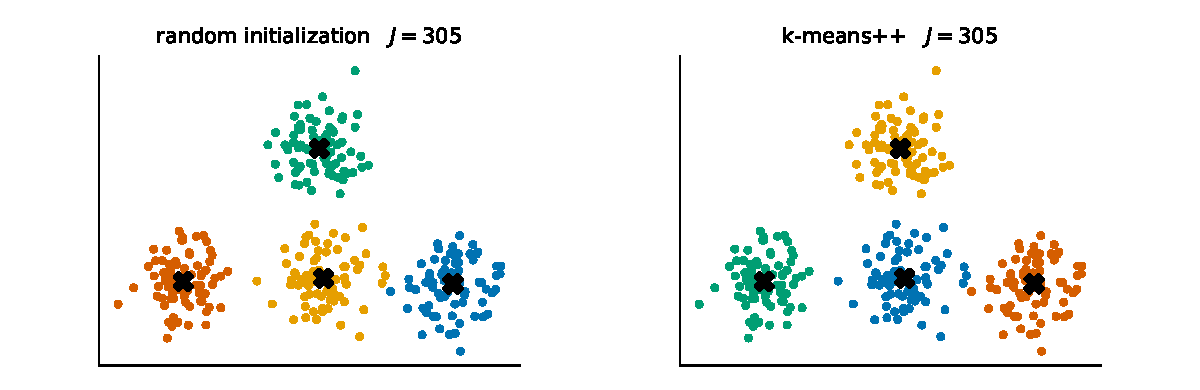
\includegraphics[height=0.24\textheight]{fig_kmeans_init.pdf}
\end{center}
\end{frame}

\begin{frame}{What $k$-Means Assumes}
$k$-means is the special case of fitting a mixture of $K$ Gaussians with identical spherical covariance
$\sigma^2\vI$ and $\sigma\to0$ --- each half-step is a hard-assignment version of the EM algorithm.
So it inherits the assumptions:
\begin{itemize}
  \item \textbf{Spherical clusters}: Euclidean distance, so elongated clusters get cut across the long axis.
  \item \textbf{Similar sizes}: a large cluster's points near a small cluster get stolen by it.
  \item \textbf{Every point belongs somewhere}: no notion of noise or outliers; one far point drags a centroid.
  \item \textbf{Scale}: change the units of one feature and every distance changes. Standardize first.
\end{itemize}
\begin{center}
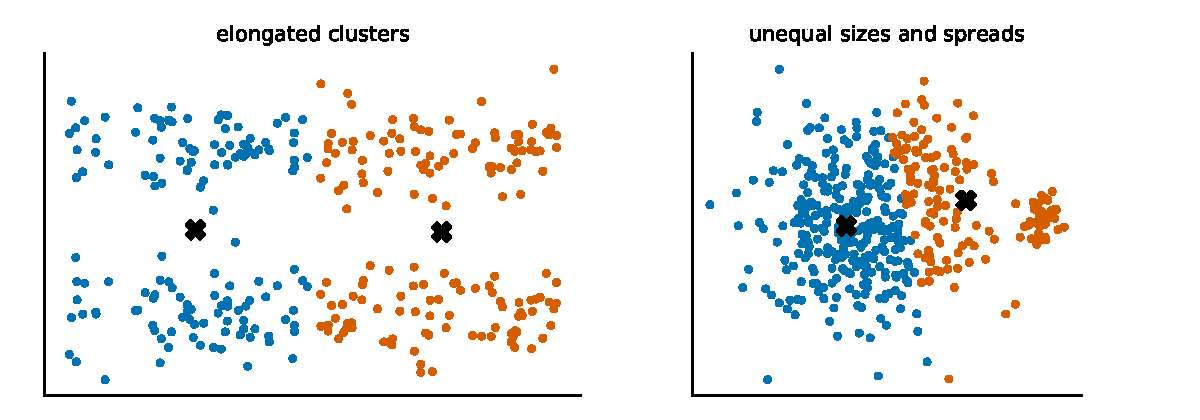
\includegraphics[height=0.32\textheight]{fig_kmeans_fails.pdf}
\end{center}
\end{frame}

% =============================================================================
\sectionframe{Hierarchical Clustering}
% =============================================================================

\begin{frame}{Agglomerative Clustering}
No $K$ up front. Start with $N$ singleton clusters; repeatedly merge the two closest; stop when one remains.
The record of merges is a \textbf{dendrogram}; cutting it at any height gives a partition.
\begin{block}{What ``closest'' means: the linkage $d(A,B)$ between clusters}
\begin{center}
\begin{tabular}{ll}
\toprule
Single & $\min_{\va\in A,\vb\in B}\norm{\va-\vb}$ --- chains through nearby points; finds elongated shapes \\
Complete & $\max_{\va\in A,\vb\in B}\norm{\va-\vb}$ --- compact, roughly equal-diameter clusters \\
Average & $\frac{1}{|A||B|}\sum_{\va,\vb}\norm{\va-\vb}$ --- a compromise \\
Ward & the increase in within-cluster sum of squares caused by merging $A$ and $B$ \\
\bottomrule
\end{tabular}
\end{center}
\end{block}
Cost $O(N^2\log N)$ in time and $O(N^2)$ in memory for the distance matrix --- fine to $N\sim10^4$, not beyond.
\end{frame}

\begin{frame}{Ward's Criterion, Derived}\footnotesize
\begin{claim}{Merging clusters $A$ and $B$ (sizes $n_A,n_B$, means $\vmu_A,\vmu_B$) increases $J$ by
$\dfrac{n_An_B}{n_A+n_B}\norm{\vmu_A-\vmu_B}^2$}
\end{claim}
\begin{derivation}{Proof}
The merged mean is $\vmu=\frac{n_A\vmu_A+n_B\vmu_B}{n_A+n_B}$. For any set $S$ with mean $\vmu_S$ and any $\vm$,
$\sum_{i\in S}\norm{\vx_i-\vm}^2=\sum_{i\in S}\norm{\vx_i-\vmu_S}^2+|S|\,\norm{\vmu_S-\vm}^2$ (expand; the cross term
vanishes because deviations from the mean sum to zero). Apply it to $A$ and $B$ with $\vm=\vmu$:
\[
\Delta J=n_A\norm{\vmu_A-\vmu}^2+n_B\norm{\vmu_B-\vmu}^2 .
\]
Now $\vmu_A-\vmu=\frac{n_B}{n_A+n_B}(\vmu_A-\vmu_B)$ and $\vmu_B-\vmu=\frac{n_A}{n_A+n_B}(\vmu_B-\vmu_A)$, so
\[
\Delta J=\frac{n_An_B^2+n_Bn_A^2}{(n_A+n_B)^2}\norm{\vmu_A-\vmu_B}^2=\frac{n_An_B}{n_A+n_B}\norm{\vmu_A-\vmu_B}^2 .\qquad\qed
\]
\end{derivation}
Ward merges the pair whose centroids are closest, \emph{weighted toward small clusters}: two singletons at distance $d$ cost $d^2/2$; two clusters of $100$ cost $50d^2$.
\end{frame}

\begin{frame}{A Dendrogram}
\begin{center}
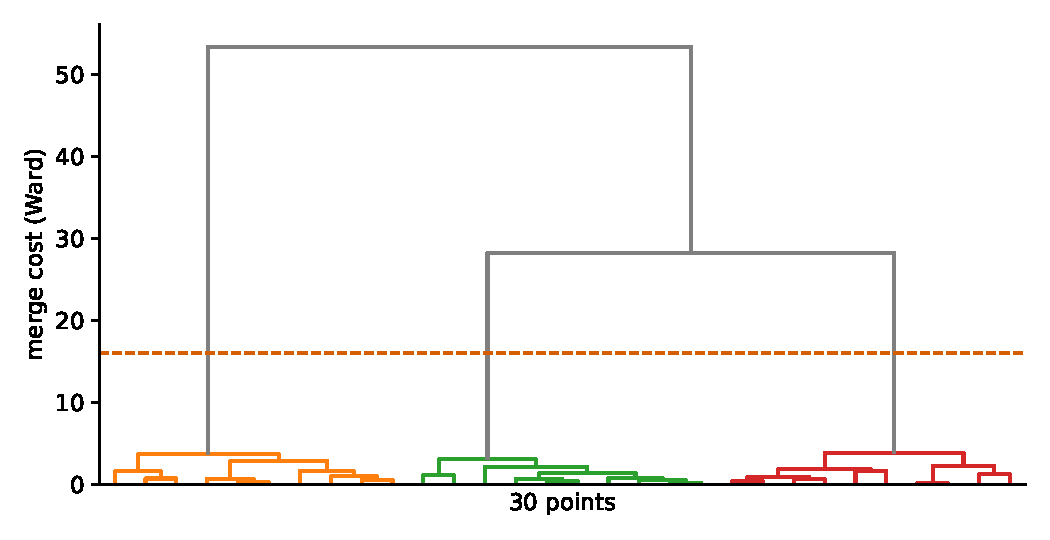
\includegraphics[height=0.62\textheight]{fig_dendrogram.pdf}
\end{center}
\vspace{-4pt}
Ward linkage on 30 points from three groups. Height = merge cost. The three long vertical stretches say that
three clusters is where the structure is; cutting at the dashed line recovers them.
\end{frame}

% =============================================================================
\sectionframe{Principal Component Analysis}
% =============================================================================

\begin{frame}{The Question}
Centre the data: $\bar\vx=\frac1N\sum_i\vx_i$, $\vx_i\leftarrow\vx_i-\bar\vx$, and stack into $\vX\in\R^{N\times p}$.
Sample covariance:
\[
\vS=\frac1N\vX\T\vX\in\R^{p\times p},\qquad\text{symmetric, positive semidefinite.}
\]
\begin{block}{Two formulations of the same question}
\begin{enumerate}
  \item \textbf{Maximum variance.} Which unit direction $\vu\in\R^p$ makes the projections $\vu\T\vx_i$ most spread out?
  \item \textbf{Minimum reconstruction error.} Which line through the origin is closest to all the points?
\end{enumerate}
\end{block}
They have the same answer. We derive it from (1), then prove (2) is equivalent.
\end{frame}

\begin{frame}{The First Principal Component}
\begin{derivation}{Maximize the projected variance}
The projection of $\vx_i$ on $\vu$ is $z_i=\vu\T\vx_i$; since the data are centred, $\bar z=0$ and
\[
\frac1N\sum_iz_i^2=\frac1N\sum_i\vu\T\vx_i\vx_i\T\vu=\vu\T\Bigl(\frac1N\vX\T\vX\Bigr)\vu=\vu\T\vS\vu .
\]
Maximize subject to $\norm\vu=1$ (otherwise scale $\vu$ up forever). Lagrangian and stationarity:
\[
\Lcal(\vu,\lambda)=\vu\T\vS\vu-\lambda(\vu\T\vu-1),\qquad
\nabla_{\vu}\Lcal=2\vS\vu-2\lambda\vu=\vzero\ \Longrightarrow\ \boxed{\vS\vu=\lambda\vu}.
\]
So $\vu$ is an eigenvector of $\vS$. At such a $\vu$ the objective is $\vu\T\vS\vu=\lambda\vu\T\vu=\lambda$.
To maximize it, take the eigenvector with the \textbf{largest eigenvalue} $\lambda_1$.
\end{derivation}
\begin{keypoint}
The first principal component is the top eigenvector of the covariance matrix, and $\lambda_1$ is the variance
along it. Both quantities are unique whenever $\lambda_1>\lambda_2$.
\end{keypoint}
\end{frame}

\begin{frame}{The Next Components}\small
Write the spectral decomposition $\vS=\vQ\vLambda\vQ\T$, $\vQ=(\vq_1,\dots,\vq_p)$ orthonormal,
$\lambda_1\ge\dots\ge\lambda_p\ge0$.
\begin{derivation}{Second component: maximize variance orthogonally to $\vq_1$}
Any unit $\vu\perp\vq_1$ expands as $\vu=\sum_{j\ge2}a_j\vq_j$ with $\sum_ja_j^2=1$, and
\[
\vu\T\vS\vu=\sum_{j\ge2}\lambda_ja_j^2\ \le\ \lambda_2\sum_{j\ge2}a_j^2=\lambda_2,
\]
with equality at $\vu=\vq_2$. By induction, the $k$-th component is $\vq_k$ with variance $\lambda_k$.
\end{derivation}
\begin{derivation}{All $k$ at once (Ky Fan): $\ \max_{\vV\T\vV=\vI_k}\tr(\vV\T\vS\vV)=\lambda_1+\dots+\lambda_k$}
Let $\vB=\vQ\T\vV$ ($p\times k$, orthonormal columns). Then $\tr(\vV\T\vS\vV)=\tr(\vB\T\vLambda\vB)=\sum_{j=1}^p\lambda_jw_j$
with $w_j=\norm{\vB_{j\cdot}}^2$ the squared norm of the $j$-th row of $\vB$. Rows of a matrix with orthonormal columns
satisfy $0\le w_j\le1$ and $\sum_jw_j=\tr(\vB\T\vB)=k$. A weighted sum of $\lambda_1\ge\dots\ge\lambda_p$ with such weights
is maximized by $w_1=\dots=w_k=1$, the rest $0$: i.e.\ $\vV=\vQ_k$, the first $k$ eigenvectors. \qed
\end{derivation}
\end{frame}

\begin{frame}{Variance $\Leftrightarrow$ Reconstruction}\footnotesize
\begin{claim}{Maximizing retained variance is minimizing squared reconstruction error}
\end{claim}
\begin{derivation}{Proof, for a $k$-dimensional subspace with orthonormal basis $\vV\in\R^{p\times k}$}
The projection of $\vx_i$ onto the subspace is $\vV\vV\T\vx_i$. By Pythagoras (Lecture 1: $\vV\vV\T$ is an orthogonal projection),
\[
\norm{\vx_i-\vV\vV\T\vx_i}^2=\norm{\vx_i}^2-\norm{\vV\vV\T\vx_i}^2=\norm{\vx_i}^2-\vx_i\T\vV\vV\T\vx_i .
\]
Sum over $i$ and divide by $N$:
\[
\underbrace{\frac1N\sum_i\norm{\vx_i-\vV\vV\T\vx_i}^2}_{\text{reconstruction error}}
=\underbrace{\frac1N\sum_i\norm{\vx_i}^2}_{\text{total variance, fixed}}
-\underbrace{\tr(\vV\T\vS\vV)}_{\text{retained variance}} .\qquad\qed
\]
\end{derivation}
Total variance is $\tr\vS=\sum_j\lambda_j$. Keeping $k$ components retains $\lambda_1+\dots+\lambda_k$ and loses
$\lambda_{k+1}+\dots+\lambda_p$. The \textbf{proportion of variance explained} is $\sum_{j\le k}\lambda_j\big/\sum_j\lambda_j$.
\end{frame}

\begin{frame}{PCA in Two Dimensions}
\begin{center}
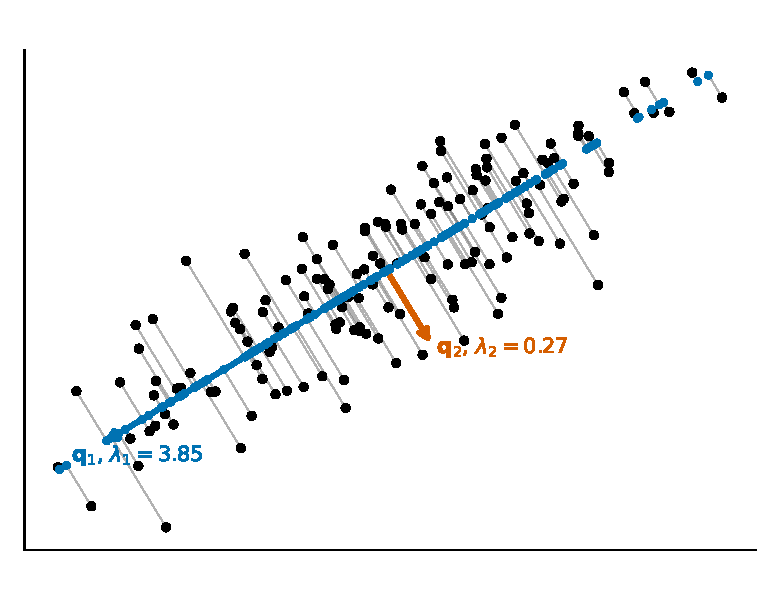
\includegraphics[height=0.6\textheight]{fig_pca_2d.pdf}
\end{center}
\vspace{-4pt}
Centred data, the two eigenvectors of $\vS$ scaled by $\sqrt{\lambda_j}$, and the projection onto $\vq_1$.
The residuals (grey) are perpendicular to $\vq_1$ --- the reconstruction-error view.
\end{frame}

\begin{frame}{PCA via the SVD}
Never form $\vS$ and diagonalize it. Take the thin SVD of the centred data matrix:
\[
\vX=\vU\vD\vV\T,\qquad\vU\in\R^{N\times p},\ \vD=\diag(d_1\ge\dots\ge d_p\ge0),\ \vV\in\R^{p\times p}.
\]
\begin{derivation}{The right singular vectors are the principal components}
\[
\vS=\frac1N\vX\T\vX=\frac1N\vV\vD\vU\T\vU\vD\vV\T=\vV\,\frac{\vD^2}{N}\,\vV\T ,
\]
which is the spectral decomposition of $\vS$ with $\vQ=\vV$ and $\lambda_j=d_j^2/N$.
\end{derivation}
\begin{itemize}
  \item \textbf{Loadings}: columns of $\vV$. \quad \textbf{Scores} (coordinates of each point on the components): $\vZ=\vX\vV=\vU\vD$.
  \item Cost $O(Np^2)$, numerically stable, and it gives the rank-$k$ truncation directly (next slide).
  \item Lecture 3's ridge shrinks direction $j$ by $d_j^2/(d_j^2+\lambda)$. \textbf{Principal components regression}
        keeps directions $1,\dots,k$ and drops the rest: a hard threshold where ridge is a soft one.
\end{itemize}
\end{frame}

\begin{frame}{Eckart--Young: The Best Low-Rank Approximation}
\begin{claim}{Theorem (Eckart--Young--Mirsky, 1936)}
Among all matrices $\vB$ of rank at most $k$, the one minimizing $\norm{\vX-\vB}_F$ is the truncated SVD
$\vX_k=\vU_k\vD_k\vV_k\T$, and the minimum is $\norm{\vX-\vX_k}_F^2=\sum_{j>k}d_j^2$.
\end{claim}
\begin{derivation}{Proof for $\vB$ of the form $\vX\vP$, $\vP$ a rank-$k$ orthogonal projection (the PCA case)}
This is the previous two slides in matrix form. Write $\vP=\vV\vV\T$ with $\vV\T\vV=\vI_k$. Then
\[
\norm{\vX-\vX\vV\vV\T}_F^2=\norm\vX_F^2-\tr(\vV\T\vX\T\vX\vV)=\sum_jd_j^2-N\tr(\vV\T\vS\vV),
\]
minimized, by Ky Fan, at $\vV=\vV_k$, giving $\sum_jd_j^2-\sum_{j\le k}d_j^2=\sum_{j>k}d_j^2$. \qed
\end{derivation}
The general statement (arbitrary $\vB$, and also the spectral norm) needs one more inequality (Weyl) and is
in \emph{ESL} \S14.5. ML II uses it constantly: it is the reason low-rank factorization works.
\end{frame}

\begin{frame}{How Many Components?}
\begin{columns}[T]
\begin{column}{0.5\textwidth}
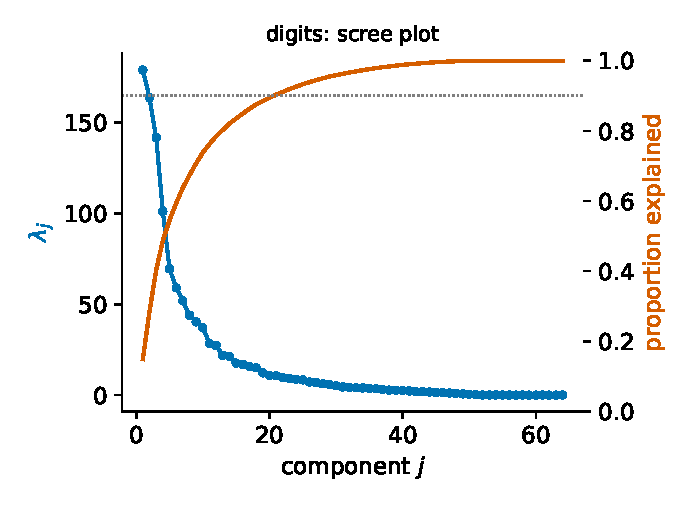
\includegraphics[width=\textwidth]{fig_scree.pdf}
\end{column}
\begin{column}{0.48\textwidth}
\begin{itemize}
  \item \textbf{Scree plot}: $\lambda_j$ against $j$. Keep components before the plot flattens.
  \item \textbf{Cumulative variance}: keep the smallest $k$ that explains, say, $90\%$.
  \item \textbf{Downstream task}: if PCA feeds a supervised model, choose $k$ by cross-validating \emph{that} model.
        The only choice with a test error behind it.
  \item Standardize first unless the features share units: PCA chases variance, and a feature in
        large units has large variance for no reason.
\end{itemize}
\end{column}
\end{columns}
\end{frame}

\begin{frame}{Eigendigits}
\begin{center}
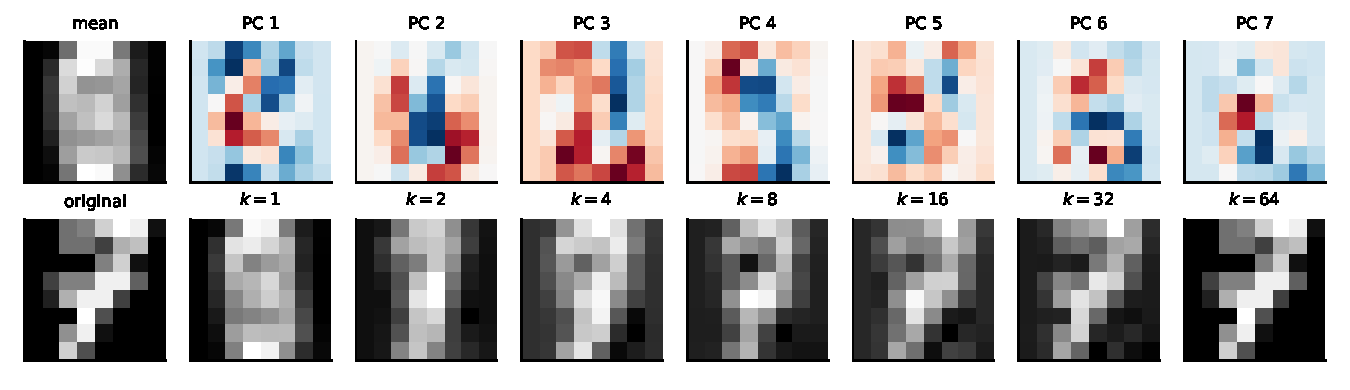
\includegraphics[width=0.92\textwidth]{fig_eigendigits.pdf}
\end{center}
\vspace{-4pt}
Handwritten digits, $8\times8=64$ pixels each. Top row: the mean and the first seven principal components,
reshaped as images. Bottom: one digit reconstructed with $k=1,2,4,8,16,32,64$ components. At $k=16$ it is
recognizable; at $k=64$ it is exact.
\end{frame}

% =============================================================================
\sectionframe{Bridge to Machine Learning II}
% =============================================================================

\begin{frame}{What PCA Really Is}
Three readings of the same $\vX\approx\vU_k\vD_k\vV_k\T$:
\begin{enumerate}
  \item \textbf{Geometry}: the best $k$-dimensional subspace, in squared distance.
  \item \textbf{Latent factors}: each observation is a combination of $k$ hidden factors, $\vx_i\approx\vV_k\vz_i$, with
        $\vz_i=\vD_k\vU_{i\cdot}\T$. The factors are unobserved; only their mixtures are.
  \item \textbf{A linear autoencoder}: encode $\vz=\vV_k\T\vx$, decode $\hat\vx=\vV_k\vz$, trained to minimize $\norm{\vx-\hat\vx}^2$.
        A neural network with one linear hidden layer of width $k$ learns exactly this subspace.
\end{enumerate}
\vspace{6pt}
Machine Learning II starts by loosening each reading in turn: latent factors with missing entries
(matrix completion), non-negative factors (NMF), then non-linear encoders and decoders --- and the word
``embedding'' will mean a learned $\vz_i$.
\end{frame}

\begin{frame}{What We Proved Today}
\begin{enumerate}
  \item $k$-means: with centroids fixed, assign to the nearest; with assignments fixed, centroids are means.
        Each half-step lowers $J$; finitely many assignments; so it terminates at a local minimum.
  \item Ward's merge cost is $\frac{n_An_B}{n_A+n_B}\norm{\vmu_A-\vmu_B}^2$.
  \item The first principal component is the top eigenvector of $\vS$ (Lagrangian); the first $k$ are the top $k$
        eigenvectors (Ky Fan); retained variance $=\lambda_1+\dots+\lambda_k$.
  \item Maximum variance $\Leftrightarrow$ minimum reconstruction error (Pythagoras).
  \item The right singular vectors of centred $\vX$ are the principal components, $\lambda_j=d_j^2/N$;
        the truncated SVD is the best rank-$k$ approximation (Eckart--Young).
\end{enumerate}
\end{frame}

\begin{frame}{Next}
\textbf{Lab 4 (Wednesday, Rodrigo)} --- $k$-means from scratch with the convergence check, Ward's formula
verified numerically, PCA by eigendecomposition and by SVD, eigendigits, and the ML I mini-project due.
\vspace{8pt}

\textbf{Machine Learning II (Friday, October 2)} --- the perceptron revisited, from the other side:
what happens when you stack linear models and put a nonlinearity between them.
\vspace{8pt}

\textbf{Reading} --- \emph{ESL} \S14.3.6 ($k$-means), \S14.3.12 (hierarchical), \S14.5.1 (PCA),
\S14.5.2--14.5.3 (SVD, low rank). Arthur \& Vassilvitskii (2007) for $k$-means++.
\end{frame}

\end{document}
